% LaTeX source for ``Complexity and Computation''
% Copyright (c)  2011  Allen B. Downey.

% Permission is granted to copy, distribute, transmit and adapt
% this work under a Creative Commons
% Attribution-NonCommercial-ShareAlike 3.0 Unported License:
% http://creativecommons.org/licenses/by-nc-sa/3.0/

% If you are interested in distributing a commercial version of this
% work, please contact Allen B. Downey.

% The LaTeX source for this book is available from
% http://greenteapress.com/complexity
% http://code.google.com/p/complexity

% This book was typeset using LaTeX .  The illustrations were
% drawn in xfig.  All of these are free, open-source programs.

%%----------------------------------------------------------------

% How to compile this document:
% If your environment provides latex, makeindex, and dvips,
% the following commands should produce a Postscript version
% of the book.

%        latex book
%        makeindex book
%        latex book
%        dvips -o book.ps book

% You will also need the following (fairly standard) latex
% packages: url, epsfig, makeidx, fancyhdr

% This distribution also includes a Makefile that should
% compile both the Postscript and PDF versions of the book.

%%-----------------------------------------------------------------

\documentclass[10pt]{book}
\usepackage[width=5.5in,height=8.0in,
  hmarginratio=3:2,vmarginratio=1:1]{geometry}

\usepackage{url}
\usepackage{fancyhdr}
\usepackage{graphicx}
\usepackage{amsmath, amsthm, amssymb}
\usepackage{exercise}
\usepackage{makeidx}
\usepackage{setspace}
\usepackage{hevea}
\usepackage{upquote}

\usepackage{soul}

\newcommand{\thetitle}{Complexity and Computation}
\newcommand{\theversion}{1.0.3}

% these styles get translated in CSS for the HTML version
\newstyle{a:link}{color:purple;}
\newstyle{p+p}{margin-top:1em;margin-bottom:1em}
\newstyle{img}{border:0px}

% change the arrows in the HTML version
\setlinkstext
  {\imgsrc[ALT="Previous"]{back.png}}
  {\imgsrc[ALT="Up"]{up.png}}
  {\imgsrc[ALT="Next"]{next.png}}

\makeindex

\begin{document}

\frontmatter

% LATEXONLY

\input{latexonly}

\newtheorem{ex}{Exercise}[chapter]

\begin{latexonly}

\renewcommand{\blankpage}{\thispagestyle{empty} \quad \newpage}

%\blankpage
%\blankpage

% TITLE PAGES FOR LATEX VERSION

%-half title--------------------------------------------------
\thispagestyle{empty}

\begin{flushright}
\vspace*{2.0in}

\begin{spacing}{3}
{\huge \thetitle}
\end{spacing}

\vspace{0.25in}

Version \theversion

\vfill

\end{flushright}

%--verso------------------------------------------------------

\blankpage
\blankpage
%\clearemptydoublepage
%\pagebreak
%\thispagestyle{empty}
%\vspace*{6in}

%--title page--------------------------------------------------
\pagebreak
\thispagestyle{empty}

\begin{flushright}
\vspace*{2.0in}

\begin{spacing}{3}
{\huge \thetitle}
\end{spacing}

\vspace{0.25in}

Version \theversion

\vspace{1in}


{\Large
Allen Downey\\
}


\vspace{0.5in}

{\Large Green Tea Press}

{\small Needham, Massachusetts}

%\includegraphics[width=1in]{figs/logo1.eps}
\vfill

\end{flushright}


%--copyright--------------------------------------------------
\pagebreak
\thispagestyle{empty}

{\small
Copyright \copyright ~2011 Allen Downey.


Printing history:

\begin{description}

\item[Fall 2008:] First edition.

\item[Fall 2011:] Second edition.

\end{description}

\vspace{0.2in}

\begin{flushleft}
Green Tea Press       \\
9 Washburn Ave \\
Needham MA 02492
\end{flushleft}

Permission is granted to copy, distribute, transmit and adapt
this work under a Creative Commons
Attribution-NonCommercial-ShareAlike 3.0 Unported License:
\url{http://creativecommons.org/licenses/by-nc-sa/3.0/}.

If you are interested in distributing a commercial version of this
work, please contact Allen B. Downey.

The original form of this book is \LaTeX\ source code.  Compiling this
\LaTeX\ source has the effect of generating a device-independent
representation of the book, which can be converted to other formats
and printed.

The \LaTeX\ source for this book is available from

\begin{verbatim}
      http://greenteapress.com/complexity
      http://code.google.com/p/complexity
\end{verbatim}

This book was typeset using \LaTeX .  The illustrations were
drawn in xfig.

The cover photo is courtesy of {\tt blmurch}, and is available
under a free license from
\url{http://www.flickr.com/photos/blmurch/2034678924/sizes/l/in/photostream/}.

\vspace{0.2in}

} % end small

\end{latexonly}




% START THE BOOK
\mainmatter

%%%%%%%%%%%%%%%%%%%%%%%%%%%%%%%
\newcommand{\TODO}{\hl{\emph{TODO:}}\hl}
%Get rid of the above when done.

\chapter{Virtual Evolution}

\section{Karl Sims}

In 1994, a researcher named Karl Sims simulated Darwinian evolution by breeding 
virtual block creatures to accomplish tasks such as running, jumping, and following 
light sources in a physical environment. His work was groundbreaking because he didn't 
start by designing a control algorithm or a body for his creatures; the creatures 
evolved complex brains and bodies {\em without human intervention}. You can look at 
some of his work on YouTube at \url{youtube.com/watch?v=JBgG_VSP7f8}. Even though 
the creatures were randomly generated, some of them look remarkably similar 
to animals in the real world, because they evolved comparably efficient  
locomotion mechanisms.
\index{Sims, Karl}
\index{Evolution, Darwinian}

In the paper\footnote{\url{karlsims.com/papers/siggraph94.pdf}} he presented at SIGGRAPH\footnote{An annual computer graphics 
conference: \url{wikipedia.org/wiki/SIGGRAPH}} 1994, Sims claimed that his work could be used to simplify the task of creating
``desirable complexity for use in virtual worlds and computer animation.'' True to this prediction, many popular computer games 
now use realtime physics simulations based on his work.\footnote{\url{aigamedev.com/open/editorial/naturalmotion-euphoria/}}

\section{Genetic Algorithms}

% TODO: Make this flow better!
Sims used {\bf genetic algorithms}, which model the process of natural evolution to solve  
problems with large solution spaces that are computationally expensive to define.
In a nutshell, a genetic algorithm operates on {\bf genotypes}, genetic material encoding {\bf phenotypes},
which represent possible solutions to a problem. As the algorithm runs, the {\em fittest} 
phenotypes survive to form a new (hopefully better) population, and the process
repeats until an end condition is reached (for example, when an optimal
solution has been found).  

More explicitly stated, a genetic algorithm consists of the following 
steps\footnote{\url{wikipedia.org/wiki/Genetic_algorithm}}:
\index{Genetic Algorithms}

\begin{enumerate}
  \item Generate an initial population of genotypes that encode potential
  phenotypes. This initial population is usually random.

  \item Evaluate the ``goodness'' of each phenotype in the population using a 
  {\bf fitness function}.

  \item Select phenotypes probabilistically such that fit phenotypes 
  are more likely to be selected.

  \item Breed the selected phenotypes by combining 
  traits of their corresponding genotypes and modifying some of them randomly through. 
  The result of this step is a new population of genotypes that will be used in
  the next generation of the algorithm.

  \item Repeat until an optimal solution has been identified, the algorithm has run for the maximum 
  number of generations, or some other terminal condition is triggered.

\end{enumerate}
\index{genotype}
\index{phenotype}
\index{fitness function}

Genetic algorithms are a subset of {\bf Evolutionary Algorithms}, which you can
read about at \url{wikipedia.org/wiki/Evolutionary_algorithm}.

How do genetic algorithms solve problems? All possible solutions to a problem
exist within a {\bf solution space} and a genetic algorithm is a type of
{\bf search algorithm} for finding the optimal solution in that space.
\index{solution space}
\index{search algorithm}

\beforefig
\centerline{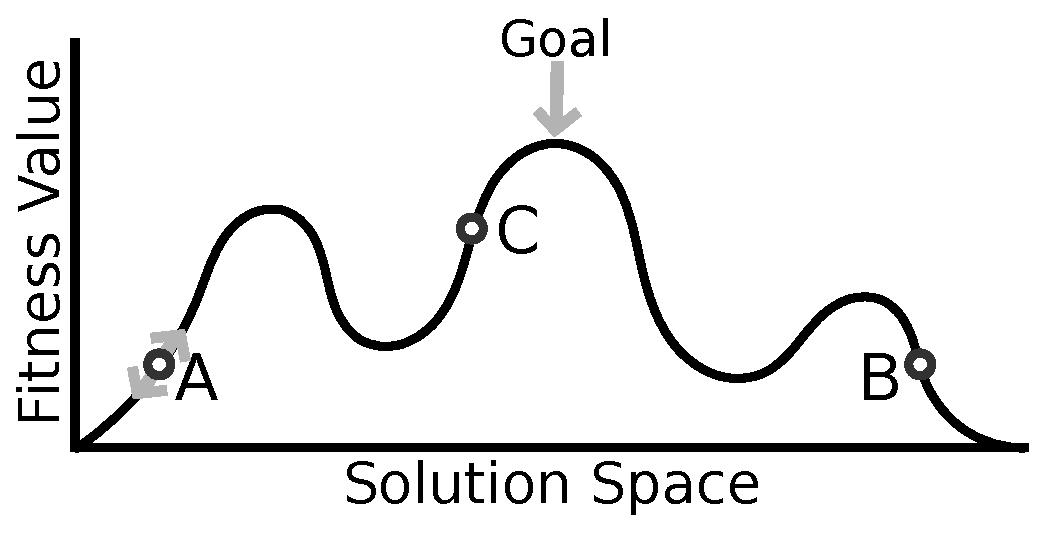
\includegraphics[width=2in]{./figs/GeneticAlgStateSpace.eps}}
\afterfig

In the diagram above, {\tt A} and {\tt B} represent randomly generated
individuals with relatively low fitness values. During breeding, there is a
chance that a trait is mutated. This usually results in a lower fitness value,
but can at times be beneficial, as the arrows around {\tt A}
indicate. Breeding between two individuals
generally involves a {\em crossover} of traits, 
with the goal of mixing good behaviors in order to create a new individual 
on a different hill in the solution space. For example, breeding {\tt A} 
and {\tt B} could result in {\tt C} in the diagram above, which is closer 
to the global maximum than either of its parents.
 
% Could be too much of a leap, TODO: decide if keep or not
\begin{ex}
  Read about the 8 queens problem at \url{wikipedia.org/wiki/8_queens}.
  Try to solve it using a genetic algorithm. Hint: you can represent
  each possible solution as a string where each character is a number
  between 0 and 7.
\end{ex}

\section{A Simple Brain Model}

Karl Sims' creatures are driven by control systems called {\bf artificial neural
networks}, which model the behavior of cells in biological brains. They 
have been used successfully to perform non-linear data analysis in fields such as
pattern matching and image recognition.
\index{neural networks}

The basic unit of computation in a neural network (NN) is the {\bf neuron}, which
roughly corresponds to a logic gate in a CPU. However, while logic gates in 
processors only deal with binary values, nodes in most NNs support real numbers.
As is shown in the example below, every neuron (or node) in a network evaluates a 
function that operates on one or more inputs to produce one or more output values. 
Each edge in the graph has a weight associated with it, which scales the value passed in: %TODO: Introduce graphs in the context on NNs
\index{neuron}

\beforefig
\centerline{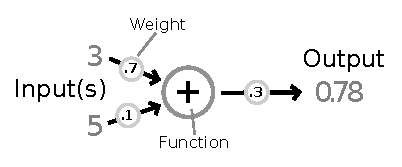
\includegraphics[width=3in]{./figs/Neuron.eps}}
\afterfig

In this example of a sum node, the input values {\tt (3,5)} yield 0.78 as the output: 
$(0.7\times 3)+(0.1\times 5) \Rightarrow 2.6$; $2.6 \times 0.3 \Rightarrow 0.78$. 
The function of a given neuron could be any operation on a set of numbers, including 
(but not limited to) difference, product, and sine. More complicated nodes can 
have a memory component. % TODO: Spell out this process

% TODO: Find a simple example of a NN that does something interesting (maybe in Braitenberg book Allen lent me) and explain how it works

% TODO: Transition from Sims to our own Implementation; what did we simplify (2d, no fluid, no competition)

% TODO: How do * we * implement the brain model?
% genotype - "graph"
% phenotype - "brain"

\section{Body Model}

% TODO: Write this section

% 1. Model (abstract - environment and cubes)
% 2. Phenotype (We are using box2d)
% 3. Genotype (How can it lead to the phenotype - example of packing and unpacking)
% 4. Introduction to mutation and crossover with examples of our own creatures

\section{PyCritters}

\TODO{Discussion of Results}
% Some things that are cool
% Some things where they take advantage of engine

\section{The Blind Watchmaker}

% TODO: Rearrange this section:
% Lead with Paley's argument
% Then go to Sims and how he refutes it
% Finally, transition to Dawkins as a fun thing to play with

As we have seen, complicated systems do not necessarily need to be designed that
way; great complexity (such as that seen in Karl Sim's virtual creatures and in the pycritters) 
can arise from simple processes. This is a counter point to the {\bf watchmaker
argument} made famous by the philosopher William Paley in 1802. 
\index{Paley, William}
\index{Watchmaker argument}

The argument follows this basic
framework\footnote{\url{wikipedia.org/wiki/Watchmaker_analogy}}:

\begin{enumerate}
  \item Watches are complex, and if you saw one, you would know that it was made
  by an {\bf intelligent designer}, a watchmaker.

  \item {\tt X}, just like a watch, is complex, where {\tt X} is an organ, a
  creature, or anything else. Therefore, it too was created by
  an intelligent designer.
\end{enumerate}

Evolutionary biologist Richard Dawkins refuted this argument in his 1986 book
{\em The Blind Watchmaker: Why the Evidence of Evolution Reveals a Universe
without Design}, in which he used the mammalian eye as an example of a complex
system that could plausibly be the product of natural selection rather than the
result of intelligent design.
\index{Blind Watchmaker@{\em The Blind Watchmaker: Why the Evidence of Evolution Reveals a Universe without Design}}
\index{Dawkins, Richard}

To further prove his point, Dawkins created a computer simulation of {\em
biomorphs}, two dimensional shapes that ``evolved'' based on user selected
mutations.\footnote{\url{wikipedia.org/wiki/The_Blind_Watchmaker}}
\index{Biomorphs}

Karl Sims' virtual creatures can be viewed as a more convincing extension of this early work by
Dawkins, because it doesn't require user interaction to create complex behavior.

\begin{ex} % TODO: Find one ourselves; give the reader clearer instructions on what to do.
  Find one of the open source implementations of Dawkins' original Biomorphs
  program, which is called {\em The Blind Watchmaker}, like his book. Can you create 
  seemingly complex shapes with it? If you have time, try to automate the selection process
  by modifying the source code. 
\end{ex}

\printindex

\clearemptydoublepage

%\blankpage
%\blankpage
%\blankpage


\end{document}
